%% ODER: format ==         = "\mathrel{==}"
%% ODER: format /=         = "\neq "
%
%
\makeatletter
\@ifundefined{lhs2tex.lhs2tex.sty.read}%
  {\@namedef{lhs2tex.lhs2tex.sty.read}{}%
   \newcommand\SkipToFmtEnd{}%
   \newcommand\EndFmtInput{}%
   \long\def\SkipToFmtEnd#1\EndFmtInput{}%
  }\SkipToFmtEnd

\newcommand\ReadOnlyOnce[1]{\@ifundefined{#1}{\@namedef{#1}{}}\SkipToFmtEnd}
\DeclareFontFamily{OT1}{cmtex}{}
\DeclareFontShape{OT1}{cmtex}{m}{n}
  {<5><6><7><8>cmtex8
   <9>cmtex9
   <10><10.95><12><14.4><17.28><20.74><24.88>cmtex10}{}
\DeclareFontShape{OT1}{cmtex}{m}{it}
  {<-> ssub * cmtt/m/it}{}
\newcommand{\texfamily}{\fontfamily{cmtex}\selectfont}
\DeclareFontShape{OT1}{cmtt}{bx}{n}
  {<5><6><7><8>cmtt8
   <9>cmbtt9
   <10><10.95><12><14.4><17.28><20.74><24.88>cmbtt10}{}
\DeclareFontShape{OT1}{cmtex}{bx}{n}
  {<-> ssub * cmtt/bx/n}{}
\newcommand{\tex}[1]{\text{\texfamily#1}}	% NEU

\newcommand{\Sp}{\hskip.33334em\relax}


\newcommand{\Conid}[1]{\mathit{#1}}
\newcommand{\Varid}[1]{\mathit{#1}}
\newcommand{\anonymous}{\kern0.06em \vbox{\hrule\@width.5em}}
\newcommand{\plus}{\mathbin{+\!\!\!+}}
\newcommand{\bind}{\mathbin{>\!\!\!>\mkern-6.7mu=}}
\newcommand{\rbind}{\mathbin{=\mkern-6.7mu<\!\!\!<}}% suggested by Neil Mitchell
\newcommand{\sequ}{\mathbin{>\!\!\!>}}
\renewcommand{\leq}{\leqslant}
\renewcommand{\geq}{\geqslant}

%mathindent has to be defined
\@ifundefined{mathindent}%
  {\newdimen\mathindent\mathindent\leftmargini}%
  {}%

\def\resethooks{%
  \global\let\SaveRestoreHook\empty
  \global\let\ColumnHook\empty}
\newcommand*{\savecolumns}[1][default]%
  {\g@addto@macro\SaveRestoreHook{\savecolumns[#1]}}
\newcommand*{\restorecolumns}[1][default]%
  {\g@addto@macro\SaveRestoreHook{\restorecolumns[#1]}}
\newcommand*{\aligncolumn}[2]%
  {\g@addto@macro\ColumnHook{\column{#1}{#2}}}

\resethooks

\newcommand{\onelinecommentchars}{\quad-{}- }
\newcommand{\commentbeginchars}{\enskip\{-}
\newcommand{\commentendchars}{-\}\enskip}

\newcommand{\visiblecomments}{%
  \let\onelinecomment=\onelinecommentchars
  \let\commentbegin=\commentbeginchars
  \let\commentend=\commentendchars}

\newcommand{\invisiblecomments}{%
  \let\onelinecomment=\empty
  \let\commentbegin=\empty
  \let\commentend=\empty}

\visiblecomments

\newlength{\blanklineskip}
\setlength{\blanklineskip}{0.66084ex}

\newcommand{\hsindent}[1]{\quad}% default is fixed indentation
\let\hspre\empty
\let\hspost\empty
\newcommand{\NB}{\textbf{NB}}
\newcommand{\Todo}[1]{$\langle$\textbf{To do:}~#1$\rangle$}

\EndFmtInput
\makeatother
%
%
%
%
%
%
% This package provides two environments suitable to take the place
% of hscode, called "plainhscode" and "arrayhscode". 
%
% The plain environment surrounds each code block by vertical space,
% and it uses \abovedisplayskip and \belowdisplayskip to get spacing
% similar to formulas. Note that if these dimensions are changed,
% the spacing around displayed math formulas changes as well.
% All code is indented using \leftskip.
%
% Changed 19.08.2004 to reflect changes in colorcode. Should work with
% CodeGroup.sty.
%
\ReadOnlyOnce{polycode.fmt}%
\makeatletter

\newcommand{\hsnewpar}[1]%
  {{\parskip=0pt\parindent=0pt\par\vskip #1\noindent}}

% can be used, for instance, to redefine the code size, by setting the
% command to \small or something alike
\newcommand{\hscodestyle}{}

% The command \sethscode can be used to switch the code formatting
% behaviour by mapping the hscode environment in the subst directive
% to a new LaTeX environment.

\newcommand{\sethscode}[1]%
  {\expandafter\let\expandafter\hscode\csname #1\endcsname
   \expandafter\let\expandafter\endhscode\csname end#1\endcsname}

% "compatibility" mode restores the non-polycode.fmt layout.

\newenvironment{compathscode}%
  {\par\noindent
   \advance\leftskip\mathindent
   \hscodestyle
   \let\\=\@normalcr
   \let\hspre\(\let\hspost\)%
   \pboxed}%
  {\endpboxed\)%
   \par\noindent
   \ignorespacesafterend}

\newcommand{\compaths}{\sethscode{compathscode}}

% "plain" mode is the proposed default.
% It should now work with \centering.
% This required some changes. The old version
% is still available for reference as oldplainhscode.

\newenvironment{plainhscode}%
  {\hsnewpar\abovedisplayskip
   \advance\leftskip\mathindent
   \hscodestyle
   \let\hspre\(\let\hspost\)%
   \pboxed}%
  {\endpboxed%
   \hsnewpar\belowdisplayskip
   \ignorespacesafterend}

\newenvironment{oldplainhscode}%
  {\hsnewpar\abovedisplayskip
   \advance\leftskip\mathindent
   \hscodestyle
   \let\\=\@normalcr
   \(\pboxed}%
  {\endpboxed\)%
   \hsnewpar\belowdisplayskip
   \ignorespacesafterend}

% Here, we make plainhscode the default environment.

\newcommand{\plainhs}{\sethscode{plainhscode}}
\newcommand{\oldplainhs}{\sethscode{oldplainhscode}}
\plainhs

% The arrayhscode is like plain, but makes use of polytable's
% parray environment which disallows page breaks in code blocks.

\newenvironment{arrayhscode}%
  {\hsnewpar\abovedisplayskip
   \advance\leftskip\mathindent
   \hscodestyle
   \let\\=\@normalcr
   \(\parray}%
  {\endparray\)%
   \hsnewpar\belowdisplayskip
   \ignorespacesafterend}

\newcommand{\arrayhs}{\sethscode{arrayhscode}}

% The mathhscode environment also makes use of polytable's parray 
% environment. It is supposed to be used only inside math mode 
% (I used it to typeset the type rules in my thesis).

\newenvironment{mathhscode}%
  {\parray}{\endparray}

\newcommand{\mathhs}{\sethscode{mathhscode}}

% texths is similar to mathhs, but works in text mode.

\newenvironment{texthscode}%
  {\(\parray}{\endparray\)}

\newcommand{\texths}{\sethscode{texthscode}}

% The framed environment places code in a framed box.

\def\codeframewidth{\arrayrulewidth}

\newenvironment{framedhscode}%
  {\parskip=\abovedisplayskip\par\noindent
   \hscodestyle
   \arrayrulewidth=\codeframewidth
   \tabular{@{}|p{\linewidth-2\arraycolsep-2\arrayrulewidth-2pt}|@{}}%
   \hline\framedhslinecorrect\\{-1.5ex}%
   \let\endoflinesave=\\
   \let\\=\@normalcr
   \(\pboxed}%
  {\endpboxed\)%
   \framedhslinecorrect\endoflinesave{.5ex}\hline
   \endtabular
   \parskip=\belowdisplayskip\par\noindent
   \ignorespacesafterend}

\newcommand{\framedhslinecorrect}[2]%
  {#1[#2]}

\newcommand{\framedhs}{\sethscode{framedhscode}}

% The inlinehscode environment is an experimental environment
% that can be used to typeset displayed code inline.

\newenvironment{inlinehscode}%
  {\(\def\column##1##2{}%
   \let\>\undefined\let\<\undefined\let\\\undefined
   \newcommand\>[1][]{}\newcommand\<[1][]{}\newcommand\\[1][]{}%
   \def\fromto##1##2##3{##3}%
   \def\nextline{}}{\) }%

\newcommand{\inlinehs}{\sethscode{inlinehscode}}

% The joincode environment is a separate environment that
% can be used to surround and thereby connect multiple code
% blocks.

\newenvironment{joincode}%
  {\let\orighscode=\hscode
   \let\origendhscode=\endhscode
   \def\endhscode{\def\hscode{\endgroup\def\@currenvir{hscode}\\}\begingroup}
   %\let\SaveRestoreHook=\empty
   %\let\ColumnHook=\empty
   %\let\resethooks=\empty
   \orighscode\def\hscode{\endgroup\def\@currenvir{hscode}}}%
  {\origendhscode
   \global\let\hscode=\orighscode
   \global\let\endhscode=\origendhscode}%

\makeatother
\EndFmtInput
%

\chapter{Future Work}
The given type system and implementation leave much to be desired.
In this chapter we provide a few different options for future work.
The idea of expressing time as part of the type system is interesting enough to produce future research.

\subsection{Solving Constraints Without \gls{smt}-solvers}
Currently we rely on \gls{smt}-solvers to both check whether the constraints hold, as well as finding suitable places to add registers.
Use of \gls{smt}-solvers offers flexibility; during development it is useful to have a very powerful tool which can handle many situations.
However, checking the generated constraints using \gls{smt}-solvers is overly complex for the situation we currently use them in.

In our current approach, we never eliminate constraints.
It may be possible to eliminate constraints when applying $\lambda$-abstraction.
When applying $\lambda$-abstraction (rule TT-Abs, def. \ref{def:tt-abs}, page \pageref{def:tt-abs}), the resulting timed type encloses both $x$ (the parameter) and $e$ (the expression used to build the abstraction).
If the time variables used in the constraints for both $x$ and $e$ are not used in an application involving the abstraction $\lambda x.e$, then these constraints should be removable.
It is difficult to see a situation where constraint can not be eliminated, other than possibly through user defined constraints (see section \ref{sec:usrcon}).
Barring those situations, if we are able to determine whether all constraints can be removed under abstraction, it would make solving of constraints trivial.
The rule TT-App (rule TT-App, def. \ref{def:tt-app}, page \pageref{def:tt-app}) is then the only way constraints can be added, as currently the only \textit{other} way is through abstraction.
As a result, the number of variables to solve for is extremely limited in the average case.
Given that abstraction removes constraints, the set of variables used in the constraints is limited, as they can only be created by successive application inside a single abstraction.
In turn, this makes simple iterative methods more feasible.

\subsection{Different Approach to Expressing Time in a Type System}
In this thesis, we used constraints as our method to express time as part of the type system.
We chose to use constraints, as they greatly simplify the process of developing a type system.
Due to constraints, we have effectively split the checking of types, from (re)constructing types.
This makes it easier to create a separate algorithm, or in our case, forgo creation of the algorithm altogether.

By using a separate algorithm for checking constraints and solving for the number of registers needed, it becomes possible to ``dynamically'' add registers in order to uphold referential transparency.
This means that function application has a side-effect, which is not apparent from the operation itself.
A bigger context is needed in order to understand the implications of function application.

This is a situation which is not very desireable, as it also increases complexity for the designer.
With a straightforward, rule-based system, it is easy to figure out why the system rejects or approves a certain expression.
When a bigger context is needed in order to reconstruct and/or typecheck an expression, it can also become more complex to understand the decisions the type (re)construction algorithm makes.
In the same vein, a possible soundness proof would also be harder to create.

To sidestep this issue, different types of type systems could be investigated.
Subtyping could be investigated by forming a subtyping relation where $a\langle t + n\rangle$ is a subtype of $a\langle t \rangle$ for some $n \in \mathbb{N}_0$.
The difficulty then is to define a subtyping relation between functions, which does not cause unreasonable effects.

Refinement types\cite{freeman1991refinement}, where function arguments can have preconditions, and function results can have post conditions, could be used to express the time constraints of functions.
Liquid types\cite{rondon2008liquid} have an implementation in the Haskell language through LiquidHaskell\cite{liquidhaskell} and could be used to eliminate our own usage of \gls{smt}-solvers.
However, LiquidHaskell also uses \gls{smt}-solvers internally, so using the refinement approach of other languages might be more interesting from a research point of view.

\subsection{Let-bindings \& Polymorphism}
Currently, our type system does not support polymorphism as used in the language ML\cite{milner1978theory} or other languages.
To introduce such polymorphism, let-polymorpishm as introduced by \citeauthor{milner1978theory} could be introduced.
First, a let binding like the one below should be created.

\begin{definitiontitled}[text only]{Typing rule for Let-bindings}{def:tt-let}
\centering
\begin{tabular}{l l}
$ \displaystyle
\frac{ C;\Gamma \vdash e_1 : \forall t_1. \tau_1 \quad C;\Gamma \vdash e_2 : \forall t_2. \tau_2
} { C;\Gamma \vdash \textbf{let } x = e_1 \textbf{ in } e_2 }
$ &
TT-Let\\
\end{tabular}
\end{definitiontitled}

However, in our type system as introduced in chapter \ref{ch:typesystem}, every different usage of $x$ in $e_2$ uses the same time variables.
Polymorphism could be added by changing the time variables at every usage.
Perhaps changing the rule TT-Gen (def \ref{def:typerules}, page \pageref{def:typerules}) to replace the time variable $t$ in $\tau$ with a fresh variable would suffice.
However, this change must also be reflected in the constraints which $e_1$ is subject to. 
It is difficult to see whether simply using $\alpha$-conversion on the constraints would work out.

Similarly, we have not defined traditional polymorphism.
The type system of \gls{clash} is pleasant to use for its use of higher order functions and polymorphism.
The supplied type system could be expanded to include polymorphism of base types.
To do so, the approach of HM(X) could be used, or the system could be extended with something similar to algorithm $W$.

\subsection{Feedback}
Even though we have described memory elements as part of the type system, we have not been able to describe the feedback operation.
The feedback operation consists of a memory element which, contrary to pipelining, feeds a value back into the circuit that produced the value.
For instance, the circuit of figure \ref{fig:mulaccstate} uses the feedback operation to create a sum of multiple multiplications.

\begin{figure}[H]
\begin{center}
\centering
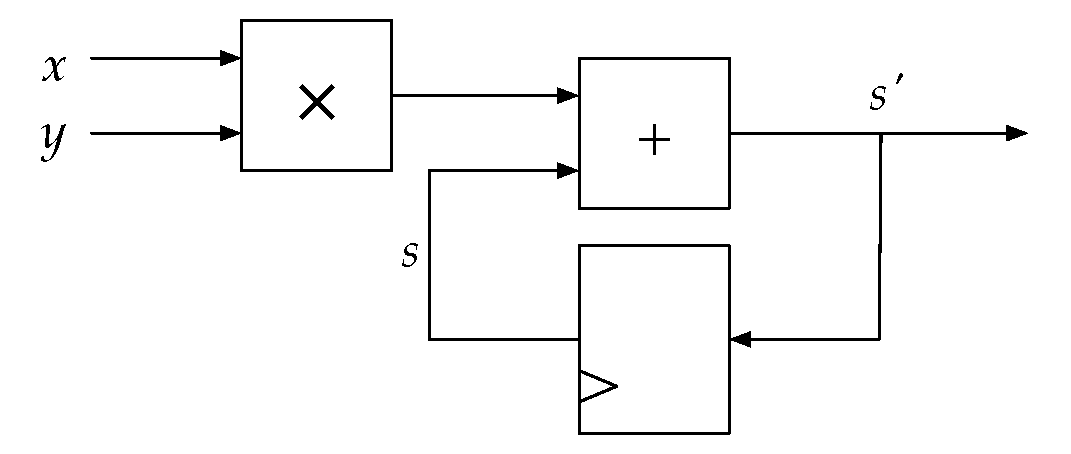
\includegraphics[width=0.6\textwidth]{images/mulaccstate}
\end{center}
\caption{Circuit of multiply-accumulate.} \label{fig:mulaccstate}
\end{figure}

Even though we have defined sequences as syntactic sugar, we are not able to use the same sequences to define feedback.
If we define a single resulting value from the feedback operation to exist at time \ensuremath{\Varid{t}}, then it depends both on the input(s) from time \ensuremath{\Varid{t}} \textit{plus} all other inputs which have had an effect on the content of the feedback register.
An obvious type for a function which represents feedback would be
\begin{changemargin}{1cm}{0cm}
\begin{expansionno}{text only}
\ensuremath{\Varid{feedback}\mathbin{::}\Conid{Int}\langle\mathrm{0}\mathinner{\ldotp\ldotp}\Varid{t}\rangle\to \Conid{Int}\langle\Varid{t}\rangle}
\end{expansionno}
\end{changemargin}
, that is, the resulting value at \ensuremath{\Varid{t}}, would depend on all values from \ensuremath{\mathrm{0}} to \ensuremath{\Varid{t}}.

The problem however, is how to define the transition from a type as \ensuremath{\Conid{Int}\langle\mathrm{0}\mathinner{\ldotp\ldotp}\Varid{t}\rangle} to \ensuremath{\Conid{Int}\langle\Varid{t}\rangle}.
Even if a way exists to describe such a transition, would it be able to accurately describe different forms of feedback?
Additional research is needed to classify different forms of feedback, and finding properties of those different classes which can be expressed by a type system.

\subsection{Multiple Clock Domains}
In this thesis, we used a single clock for entire circuits.
However, for many areas in \gls{dsp}, multiple clock domains are used.
We focus on clock domains which have different speeds, but are synchronised (e.g. the clocks do not drift).

Extending the current type-system with multiple clocks is difficult, as polytemporal types only allows a single time variable in its binder.
Either multiple time variables need to be used in order to reason about different clocks, or the relation between different clocks can be mapped to time variables in a different set of constraints.
The latter would surely make the type system very complex, making it hard to reason about the system and its soundness.
The former is also difficult, as currently the single time variable used in a polytemporal type is necessary for expressing our typing rules (page \pageref{def:typerules}).

\subsection{User defined Constraints} \label{sec:usrcon}
The constraints of our type system are currently used to reason about the compositions of time-dependent behaviour.
However, time constraints could also possibly be used to verify whether restrictions imposed on the circuit from the environment are adhered to.
For instance, two functions could be defined, both with time variables in a different scope, together with a global constraint that the time variables used by those two functions are always equal.
This would then create an additional constraint which has to be adhered to no matter how these functions are used.

\subsection{Inferred Register Placement}
Currently we do not provide an algorithm which, given a set of terms and types belonging to those terms, can determine where memory elements ought to be placed.
In this thesis we only discussed placement of memory elements very briefly, only to indicate that it should \textit{in principle} be possible.
Since the type system shows possibilities with regards to retiming, an approach which determines whether retiming is intended by the designer would be more than welcome.

\subsection{Multiple Time Variables}
We only use a single time variable to define a polytemporal type.
A single time variable is needed in order to be able to reason about the effects of time expressions under abstraction and application.
However, having more than one time variable would open up many possibilities to describe more general temporal functions.
Unfortunately, having multiple time variables makes it hard to reason about functions and their temporal constraints.
As such, this option should preferably be researched together with a different approach to expressing time as part of the type system.

